\documentclass[a4paper,12pt]{article}
\usepackage[utf8]{inputenc}
\usepackage{hyperref}
\usepackage{graphicx}
\usepackage{listings}
\usepackage{xcolor}

% Configuración de código
\lstset{
    basicstyle=\ttfamily\footnotesize,
    keywordstyle=\color{blue},
    stringstyle=\color{red},
    commentstyle=\color{green},
    breaklines=true,
    frame=single
}

\title{Scraping de citas con Python y el patrón Strategy}
\author{Enrique López García}
\date{\today}

\begin{document}

\maketitle

\section{Introducción}
En esta práctica se ha implementado un programa en Python para extraer información de la web \url{https://quotes.toscrape.com/} utilizando el patrón de diseño \textbf{Strategy}. 
El objetivo es obtener las citas, autores y etiquetas de las primeras 5 páginas de la web, utilizando dos estrategias de scraping: 
\begin{itemize}
    \item \textbf{BeautifulSoup}: Analiza el HTML de la página directamente con la biblioteca BeautifulSoup.
    \item \textbf{Selenium}: Carga dinámicamente la página y extrae el contenido utilizando un navegador automatizado.
\end{itemize}

El programa permite elegir entre ambas estrategias, guarda los datos en un archivo YAML y finaliza cuando el usuario lo decide.

\section{Patrón Strategy e Implementación}
El \textbf{patrón Strategy} permite definir una familia de algoritmos, encapsularlos y hacerlos intercambiables sin modificar el código del programa principal. En este caso, el scraping se implementa con dos estrategias diferentes:

\begin{itemize}
    \item \textbf{Clase Abstracta}: Define la estructura común a ambas estrategias.
    \item \textbf{BeautifulSoupScraper}: Implementa la extracción de datos con la biblioteca BeautifulSoup.
    \item \textbf{SeleniumScraper}: Utiliza Selenium para cargar dinámicamente las páginas y extraer los datos.
    \item \textbf{ScraperContext}: Administra la estrategia seleccionada y coordina la extracción de las páginas.
\end{itemize}

\begin{figure}
    \centering
    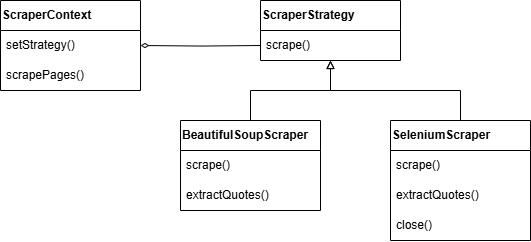
\includegraphics[width=0.75\textwidth]{images/DiagramaP1Ej3.png}
    \caption{Diagrama Implementado}
    \label{fig:diagrama_ej3}
\end{figure}


El usuario puede elegir qué estrategia usar pulsando una tecla (`B` para BeautifulSoup, `S` para Selenium, `Q` para salir).

\section{Dependencias y Funciones}
Para la realización de esta práctica se han utilizado las siguientes dependencias:

\begin{itemize}
    \item \textbf{requests}: Para hacer peticiones HTTP a la página web.
    \item \textbf{BeautifulSoup4}: Para analizar y extraer datos del HTML.
    \item \textbf{Selenium}: Para cargar dinámicamente la web y extraer el HTML.
    \item \textbf{PyYAML}: Para guardar los datos extraídos en formato YAML.
    \item \textbf{webdriver-manager}: Para gestionar automáticamente el driver de Selenium.
\end{itemize}

La información, funciones y recomendaciones necesarias para la realización de este ejercicio han sido obtenidas a través de la documentación oficial de las librerías utilizadas, recursos disponibles en Internet y el apoyo puntual de \textbf{ChatGPT} para resolver dudas específicas.

\section{Funcionamiento del Algoritmo}
El algoritmo sigue los siguientes pasos:

\begin{enumerate}
    \item Muestra un menú para seleccionar la estrategia:
    \begin{itemize}
        \item `S` → Selenium
        \item `B` → BeautifulSoup
        \item `Q` → Salir
    \end{itemize}
    
\item Extrae información de las primeras 5 páginas de \url{https://quotes.toscrape.com/}:

\begin{itemize}
    \item En cada iteración, el programa construye la URL correspondiente a cada página con el formato \texttt{https://quotes.toscrape.com/page/\{n\}/}, donde \texttt{n} va del 1 al 5.
    
    \item Si se ha seleccionado la estrategia \textbf{BeautifulSoup}, se utiliza la función \texttt{requests.get()} para descargar el HTML de la página como texto. Luego, se usa \texttt{BeautifulSoup} para parsear el HTML y acceder a los elementos necesarios mediante selectores CSS (como clases).
    
    \item En cambio, si se selecciona la estrategia \textbf{Selenium}, se lanza un navegador (de forma oculta usando modo headless) y se accede a la página cargándola completamente, como lo haría un usuario. 
    Se accede directamente al árbol DOM de la página usando funciones como \texttt{find\_elements(By.CLASS\_NAME, ***)} para ir localizando los elementos correspondientes. 

    \item Cada cita se guarda como un diccionario con tres claves: \texttt{text}, \texttt{author} y \texttt{tags}. Todos los diccionarios se almacenan en una lista que representa todas las citas extraídas.
\end{itemize}    
    \item Guarda los datos en un YAML llamado \texttt{quotes.yaml}.
    
    \item Imprime en consola las primeras 5 citas extraídas.
    
    \item Vuelve a pedir una opción al usuario hasta que pulse `Q` para salir.
\end{enumerate}

\section{Formato de Guardado y Controles del Script}
Los datos extraídos se guardan en un archivo llamado \texttt{quotes.yaml}, en formato diccionario:

\begin{lstlisting}[language=yaml]
- author: "Albert Einstein"
  text: "The world as we have created it is a process of our thinking..."
  tags: ["change", "deep-thoughts", "thinking"]
- author: "J.K. Rowling"
  text: "It is our choices, Harry, that show what we truly are..."
  tags: ["abilities", "choices"]
\end{lstlisting}


\section{Conclusión}

Tras la implementación y evaluación comparativa de ambas estrategias de scraping, se han podido extraer las siguientes conclusiones:

\begin{itemize}
    \item La estrategia basada en \textbf{BeautifulSoup} presenta un rendimiento significativamente superior en términos de velocidad. Esto se debe a que trabaja directamente sobre el contenido HTML estático obtenido mediante peticiones HTTP, sin necesidad de cargar ni renderizar un navegador.
    
    \item Por su parte, la estrategia con \textbf{Selenium} ofrece una mayor versatilidad, ya que permite interactuar con páginas que requieren ejecución de JavaScript u otros elementos dinámicos. No obstante, esta flexibilidad conlleva un mayor coste computacional y un tiempo de ejecución más elevado, debido a la inicialización del navegador y la espera a que el contenido se cargue completamente.
\end{itemize}

En el contexto de esta práctica, dado que la página web analizada no contiene contenido dinámico, la utilización de BeautifulSoup resulta más eficiente y adecuada.


\end{document}
